\chapter{Methodology}
\label{chap:methods}
In figure~\ref{fig:diagram} we present a block diagram of the whole system from where we can see that four separate stages of this thesis can be defined: data acquisition (guitar recording), transcription, feature extraction and models computation. Expressive hexaphonic guitar recordings will be done using the Roland GK-3 divided pick-up, which is able to separate sound from each string~\cite{Angulo2016}. The main output of this first stage will be a new dataset consisting of hexaphonic recordings recorded by a guitar player with different performance actions of the performance. 

\begin{figure}[ht!]
\caption{Block diagram of the whole system.}
\label{fig:diagram}
\centering
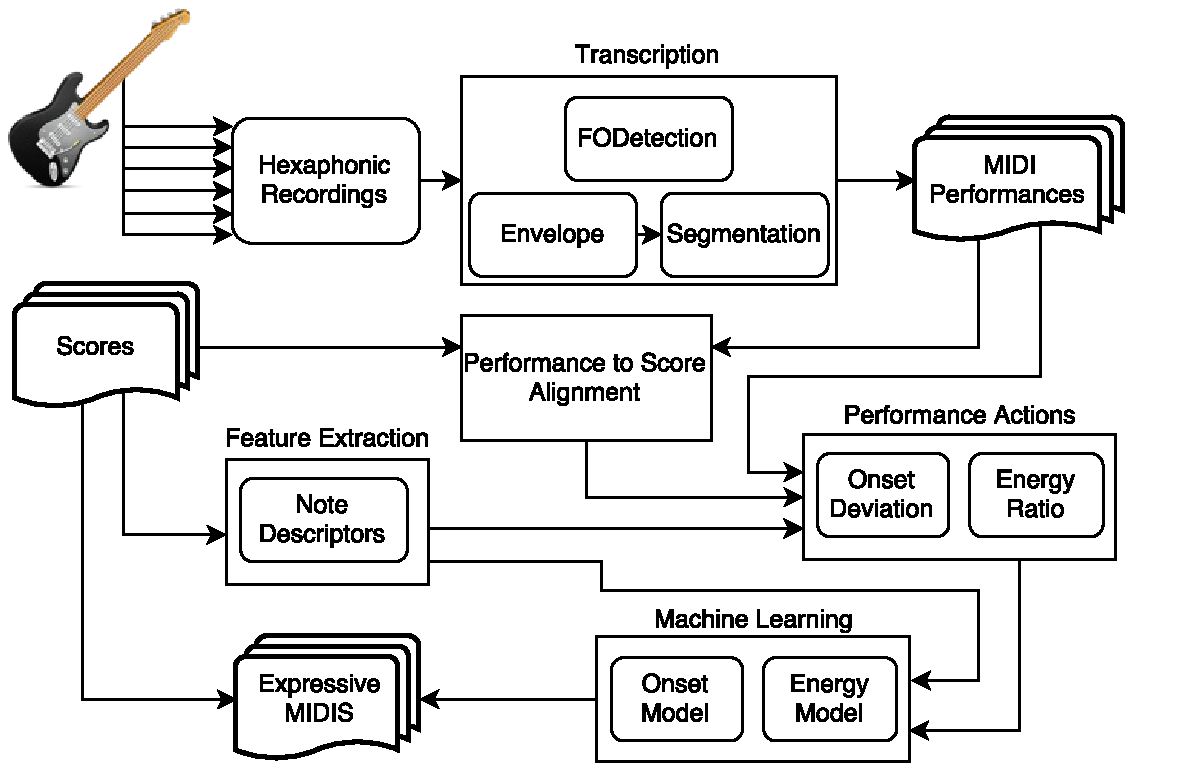
\includegraphics[width=\textwidth]{Figures/Diagram.pdf}
\end{figure}

After this step, transcription of each individual string will be computed applying non-negative matrix factorization~\cite{OGrady2009}. After doing a score alignment with the original score and the transcription of the expressive guitar performance, feature extraction needs to be done.

Feature extraction will be performed following an approach in which each note is characterized by its \textit{nominal}, \textit{neighbouring}, and \textit{contextual} properties.  Here is where the most of the research in this thesis will take place:  checking for literature in expressive piano modelling, combining it with previously mentioned features of monophonic expressive guitar modelling,... Afterwards, several machine learning and feature selection algorithms will be applied to predict those performance actions (timing, pitch, energy,...) and ornaments introduced by the musician when performing a musical piece.

\section{Data acquisition}
In order to obtain hexaphonic recordings and get each string nicely separated we used the Roland GK-3 divided pick-up that is easily attached to any steel-stringed electric guitar and acts as a sound transducer device. It is able to separate very good the sound from each string and delivers accurate performance data.

However, the output of this pick-up consists of a 13 pin DIN cable that allows to connect the guitar to guitar synthesizers such as Roland's popular GR-55 and at the same time to fed electrically the pick-up. So, in order to be able to record each string separately we need to adapt the pick-up output so the sound of each string can be inputted to the computer through an independent input channel of an audio interface.

To do this, a Breakout Box circuit was built by I.Angulo~\cite{Angulo2016} for his master's thesis last year so we reused it. The final box has an input for the 13 pin DIN cable and 6 separate Jack connector cables are outputted, one for each string. Also, two batteries are needed inside the box in order to fed the pick-up. 

In this study, the final data set consists of 3 audio recordings (one recording of \textit{Darn that dream} by Jimmy Van Heusen and Eddie De.Lange and two recordings of \textit{Suite en La} by Manuel M. Ponce) resulting in a total of 1414 notes recorded by an amateur guitarist and their corresponding music scores saved as xml file using Muse Score 2. Each of these notes was characterized by a set of descriptors as explained in the following sections.  

\section{Hexaphonic guitar transcription}
The aim of this section is to obtain machine readable (and understandable) representation from the audio recordings in order to be able to compute descriptors and performance actions. So, the audio signal from each string from the guitar was automatically transcribed into a MIDI format, in order to obtain a note representation based on pitch, onset, duration and offset for each note. This step was based on the previous work of Bantula, Giraldo and Ramírez~\cite{bantula2016}. However, the algorithm has been modified a bit in order to correctly transcribe the hexaphonic audio (that contain lickage from the other strings) instead of simple monophonic ones.

For doing this, we first need a fundamental frequency detection in order to obtain the pitch of each string. The original algorithm used the YIN algorithm~\cite{Cheveigne2002}, however, in order to improve the system we changed it to Melodia which offers more robustness against the lickage from other strings and helps to detect the main pitch present in the signal. In order to provide a better F0 detection, we also tuned the parameters of this algorithm. The minimum and maximum frequency (the range) of the detector was set differently to each string according to the frequencies that a guitar can produce. As can be seen in table~\ref{tab:guitar_strings} we considered from each string a range of one octave because in this particular recordings and scores the guitarist never passes the twelfth fret.

\begin{table}[ht!]
\centering
  \caption[Guitar Strings Frequencies.]{Guitar Strings Frequencies. Frequency refers to the base frequency of the string. MIDI refers to MIDI note number and Range to the Frequency range in Hz considered for transcription.}
  \label{tab:guitar_strings}
  \begin{tabular}{  l r c c r }
    \hline
	String & Frequency & Pitch & MIDI & Range\\ \hline
    1 (E') & 329.63 Hz & E4 & 64 & [320-660]\\ 
    2 (B) & 246.94 Hz & B3 & 59 & [240-500]\\
    3 (G) & 196.00 Hz & G3 & 55 & [190-400]\\
    4 (D) & 146.83 Hz & D3 & 50 & [140-300]\\
    5 (A) & 110.00 Hz & A2 & 45 & [100-230]\\
    6 (E) & 82.41 Hz & E2 & 40 & [80-170]\\
    \hline
  \end{tabular}

\end{table}

The power envelope of the signal is used to apply an adaptive noise gate in order to filter out none pitched sounds. That power envelope was also used in order to compute MIDI velocity (energy was linearly mapped to a value from 0 to 127). Finally, the filtered frequency pitch profile obtained is rounded to a MIDI note number.

In figure~\ref{fig:transcription} we can see the four stages of the process: we start from the audio (a), we obtain a pitch profile using Melodia (b) and using an adaptative threshold over the audio wave envelope (c) we obtain a filtered pitch profile.

Following the algorithm proposed by Bantula, a rule based filter is applied in order to remove short notes and gaps merging them with corresponding neighbour notes based on a cognitive perspective of the perception of time.

\begin{figure}[ht!]
\caption{One string automatic transcription}
\label{fig:transcription}
\centering
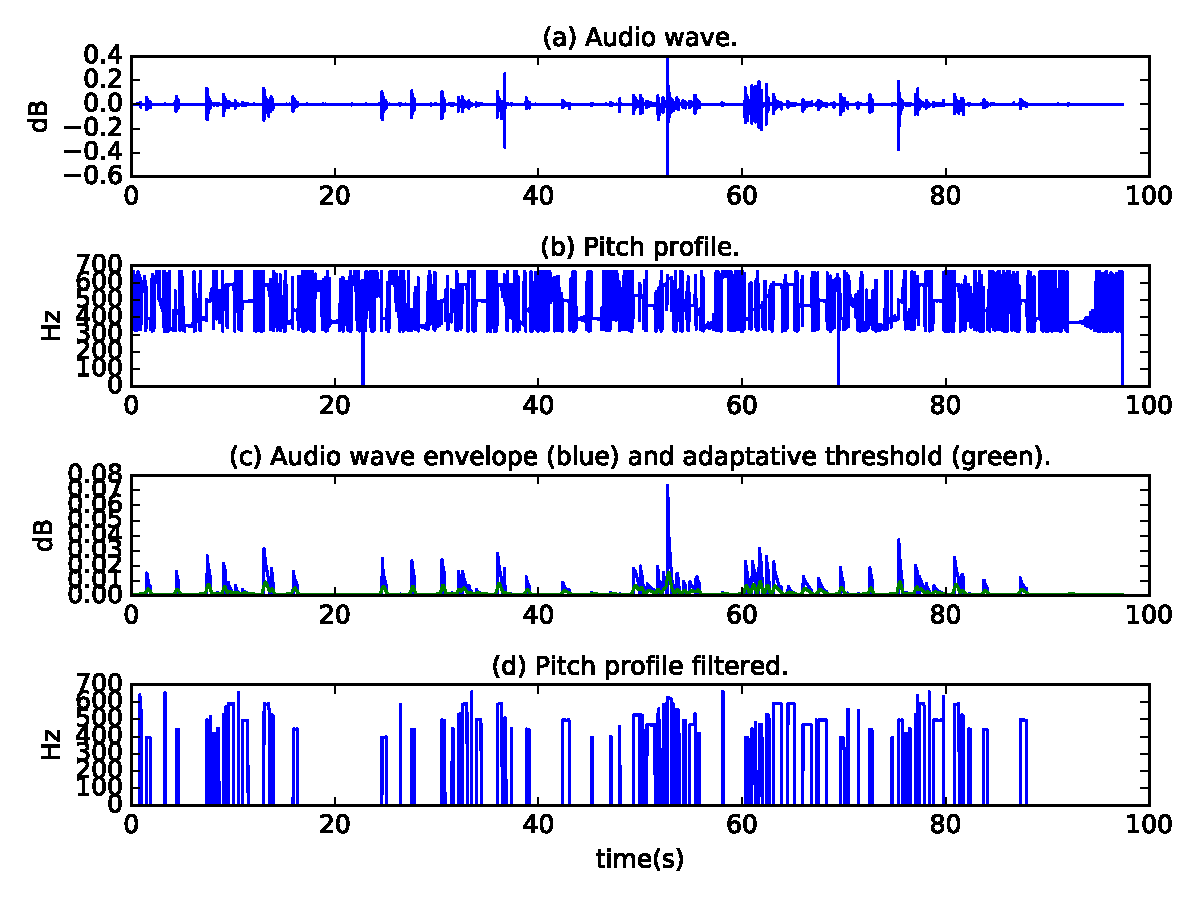
\includegraphics[width=\textwidth]{Figures/transcription.pdf}
\end{figure}

Following previous step, onsets and offsets are detected from differentiating the cleaned pitch profile. This means for a pitch remove next one, so the changes in pitch become positive or negative peaks. Positive ones (above a threshold) are labelled as onsets and negative ones (below a threshold) are labelled as offsets. Duration is computed by subtracting the offset to the onset.

After all this process, a few manual corrections were performed by changing pitch, eliminating notes or time stretching the performance in order to have a better alignment with the score. Afterwards, all six transcriptions (one from each string) were merged in order to obtain a single MIDI file from the performance. MIDI channel was used in order to label the notes according to the string where were played.

\section{Feature extraction}
In this section we describe how we analysed the music scores in order to extract multiple descriptors for each note. Afterwards, performance to score alignment was computed and performance actions such as onset deviation or energy ratio were extracted.

\subsection{Note Descriptors}
Feature extraction from the music scores was performed following an approach similar to that of Giraldo~\cite{Giraldo2016} but extended and computationally adapted to polyphonic scores, in which each note is characterized by its \textit{nominal}, \textit{neighbouring} and \textit{contextual} properties, taking into account both horizontal (time or melodic) and vertical (simultaneous or harmonic) axis. The complete list of the descriptors extracted from the music scores can be found in Table~\ref{tab:note_descriptors}.

\begin{table}
\centering
  \caption[Complete list of descriptors extracted from music scores.]{Complete list of descriptors extracted from music scores.}
  \label{tab:note_descriptors}
   \makebox[\textwidth][c]{
  \footnotesize
  \begin{tabular}{l l c c c p{2.5cm} }
    \hline 
    Code & Descriptor & Abbreviation & Units & Formula & Range \\ \hline
    
	7 & Duration & $ds_n$ & Seconds & $ds_0$ & [0,+$\infty$] \\
    2 & Duration & $db_n$ & Beats & $db_0$ & [0,+$\infty$] \\
 	6 & Onset & $ons_n$ & Seconds & $os_0$ & [0,+$\infty$] \\
 	1 & Onset & $onb_n$ & Beats & $ob_0$ & [0,+$\infty$] \\
 	15 & Onset in bar & $obm_n$ & Beats & $ob_0\%bpb$ & [0,+bpb] \\
 	4 & Pitch & $p_n$ & Semitones & $p_0$ & [1,127] \\
 	16 & Chroma & $ch_n$ & Semitones & $p_0\%12$ & [0,11] \\
 	5 & Energy & $v_n$ & MIDI vel & $v_0$ & [1,127] \\ 
    3 & String & $str_n$ & String num & $channel_0$ & [1,6] \\\hline 
    
	10 & Prev. duration & $pds_n$ & Seconds & $ds_{-1}$ & [0,+$\infty$] \\
 	9 & Prev. duration & $pdb_n$ & Beats & $db_{-1}$ & [0,+$\infty$] \\
    12 & Next duration & $nds_n$ & Seconds & $ds_1$ & [0,+$\infty$] \\
    11 & Next duration & $ndb_n$ & Beats & $db_1$ & [0,+$\infty$] \\
    18 & Prev. interval & $pint_n$ & Semitones & $p_{-1}-p_0$ & [-60,60] \\
 	19 & Next interval & $nint_n$ & Semitones & $p_1-p_0$ & [-60,60] \\
 	13 & Prev. inter-onset dist. & $piod_n$ & Seconds & $os_0-os_{-1}$ & [0,+$\infty$] \\
 	14 & Next. inter-onset dist. & $piod_n$ & Seconds & $os_1-os_0$ & [0,+$\infty$] \\
 	28 & Narmour & $nar1_n$ & Label & $nar(p_{-1},p_0,p_1)$ & [P, D, R, ID]\\
    29 & & $nar2_n$ &  & $nar(p_{-2},p_{-1},p_0)$ & [VR, IR, VP, IP] \\
	30 & & $nar3_n$ & & $nar(p_0,p_1,p_2)$ & [dyadic, monadic, none] \\
    33 & Is a Chord & $ich_n$ & Boolean & $isChord_0$ & \{true, false\} \\
    34 & Is a Pedal & $pdl_n$ & Boolean & $pdl_0$ & \{true, false\} \\
    17 & Simultaneous notes & $sim_n$ & Number & $simult_0$ & [0,+$\infty$] \\ \hline
    
    8 & Measure & $m_n$ & Bars & $m_0$ & [0,+$\infty$] \\
    31 & Tempo & $t_n$ & Bpm & $t_0$ & [30,260] \\
    20 & Key & $k_n$ & Semitones & $k_0$ & [-6,6] \\
 	35 & Mode & $mod_n$ & Label & $mod_0$ & \{major, minor\} \\
 	23 & Chord root & $chr_n$ & Semitones & $chr_0$ & [0,11] \\
    24 & Chord type & $cht_n$ & Label & $cht_0$  & \{+, 6, 7, 7\#11, 7\#5, 7\#9, 7alt, 7$\flat$5, 7$\flat$9, Maj7, dim, dim7, m, m6, m7, m7$\flat$5, major\} \\
    21 & Note to key & $n2k_n$ & Semitones & $ch_0-k_0$ & [0,11] \\
	25 & Note to chord & $n2ch_n$ & Semitones & $ch_0-chr_0$ & [0,11] \\
 	26 & Is chord note & $ichn_n$ & Boolean & $isChNote$ & \{true, false\} \\
 	27 & Metrical strength & $mtr_n$ & Label & $metStr_0$ & \{Very strong, Strong, Weak, Very weak\} \\
 	32 & Phrase & $ph_n$ & Label & $phrase_0$ & \{initial, middle, final\} \\
 

    \hline

  \end{tabular}
  }
\end{table}


\begin{itemize}
\item \textbf{Nominal}: This descriptors refer to the intrinsic or intra-note properties of score notes. So to say, this descriptors are needed in term to define completely a note. \textit{Duration} (computed from offset and onsets) and \textit{onset} are given both in seconds and beats, as the descriptor in seconds depends on the tempo of the piece. \textit{Onset in bar} refers to the position of the onset related to the beats per bar measure. If its 1 the first beat on the bar, and so on. The \textit{pitch} is directly the MIDI note number, and the \textit{chroma} is the pitch modulus 12, so to say, the pitch class of the note, the pitch without taking into account octave changes. Energy descriptor gives us how loud is the note played (the loudness), and its directly taken from MIDI velocity (how fast the note is played). Finally, \textit{string} number is also extracted for each note directly from the MIDI channel.

\item \textbf{Neighbouring}: This neighbouring or inter-note descriptors refer to the relations of the note with its neighbouring or simultaneous notes. Each note is characterized by the \textit{Previous duration} and \textit{Next duration} given both in seconds and beats. Also \textsc{Previous interval} and \textit{Next interval} is given in semitones. \textit{Inter-onset distance} refers to the onset difference between current and previous or next note. \textit{Simultaneous notes} counts the number of simultaneous notes to the current note within a given thresholds.

Following the work of Bantula~\cite{bantula2016} on piano polyphonic music, notes have been also labelled as \textit{chord notes} or \textit{pedal notes} depending on the simultaneity of other notes, differentiating between notes that have been played at the same time as a chord and notes that are played as a basis in order to have a melody in top of them.

In this neighbouring category of descriptors, categorization based on the implication-realization (I-R) model of \textit{Narmour} has been computed.  This model parses melodies and obtains for each note a label depending on the previous and next notes. This computation has also been adapted in order to take into account polyphonic melodies. 

\item \textbf{Contextual}: This descriptors refer to the context, background or properties of the song in which the note appears on. Some of this descriptors, such as \textsc{measure}, \textit{tempo}, \textit{key} or \textit{mode}, are the same for the whole song but may be useful if we merge different datasets into one. \textit{Chord root} and \textit{chord type} refer to the actual chord of that note (labelled manually per bar or per measure in the score).

Others of this descriptors are just computations of the note respecting those first. \textit{Note to key} and \textit{note to chord} refer to the distance in semitones of the actual note both to the general key root of the piece or to the actual chord root. \textit{Is chord note} gives us a boolean label depending if the note is part of those notes pre-defined by the chord root and type as can bee seen in table~\ref{tab:chord_extensions}. \textit{Metrical strength} categorize notes occurring at strong or weak beats within a bar. And \textit{phrase} descriptor labels notes depending on the melodic segmentation approach by Cambouropulos~\cite{Cambouropoulos1997a} into initial, middle and final notes.

\end{itemize}

\begin{table}[ht!]
\centering
  \caption[Chord description.] {Chord description. A list of chords definitions.  The numbers on the Intervals column indicate the index of the notes belonging to the chord, (zero indexed, in 12 semitones).}
  \label{tab:chord_extensions}
  \begin{tabular}{  l  c  l }
    \hline
    Chord type & Intervals & Example (C as root) \\ \hline
    M (major) & 0 4 7 & C E G \\
    m (minor) & 0 3 7 & C E$\flat$ G \\
    2 (sus2) & 0 2 7 & C D G \\
	sus (sus4) & 0 5 7 & C F G \\
    dim & 0 3 6 &  C E$\flat$ G$\flat$\\
    + (Aug) & 0 4 8 & C E G$\sharp$ \\
	Maj7 & 0 4 7 11 & C E G B \\
	6 (6th) & 0 4 7 9 & C E G A \\
	m7 & 0 3 7 10 & C E$\flat$ G B$\flat$ \\
	m6 & 0 3 7 9 & C E$\flat$ G A \\
	mMaj7 & 0 3 7 11 & C E$\flat$ G B \\
    m7$\flat$5 & 0 3 6 1 0& C E$\flat$ G$\flat$ B$\flat$ \\
    dim7 & 0 3 6 9 & C E$\flat$ G$\flat$ A \\
	7 (7th) & 0 4 7 10 & C E G B$\flat$ \\
	7\#5 & 0 4 8 10 & C E G$\sharp$ B$\flat$ \\
	7$\flat$5 & 0 4 6 10 & C E G$\flat$ B$\flat$ \\
	7sus & 0 5 7 10 & C F G B$\flat$ \\
	Maj9 & 0 2 4 7 11 & C D E G B \\
	69 (6/9) & 0 2 4 7 9 & C D E G A \\
	m9 & 0 2 3 7 9 & C D E$\flat$ G A \\
	9 (9th) & 0 2 4 7 10 & C D E G B$\flat$ \\
	7$\flat$9 & 0 1 4 7 10 & C D$\flat$ E G B$\flat$ \\
	7\#9 & 0 3 4 7 10 & C D$\sharp$ E G B$\flat$ \\
	13 (13th) & 0 2 4 7 9 10 & C D E G A B$\flat$ \\
	7$\flat$9$\flat$13 & 0 1 4 7 8 10 & C D$\flat$ E G A$\flat$ B$\flat$ \\
	7alt & 0 1 3 4 6 8 10 & C D$\flat$ E$\flat$ E G$\flat$ A$\flat$ B$\flat$ \\
    \hline
  \end{tabular}

\end{table}


\subsection{Performance to score alignment}

In this stage, and in order to compute performance actions in the next step, we need to know which notes on the performance correspond to which notes in the score, or mostly known as performance to score alignment.

This is done automatically and in this case we will use Dynamic Time Warping (DTW) techniques in order to match performance notes to score. Those notes are alignment depending on a cost function based on onset, pitch and duration deviations. All these deviations can be weighted with a parameter in order to penalize more errors in pitch than in onset i.e. firstly, and previously to applying DTW, performances have been manually time-stretched in order to obtain a better automatic alignment. Then we compute a cost or similarity matrix of the notes on the performance against score notes. As we can see in figure~\ref{fig:suite_cost_matrix} after the cost matrix computation, an optimal path is retrieved in order to found the alignment with less global cost.

\begin{figure}[ht!]
\caption{\textit{Suite en La} similarity matrix with optimal path,}
\label{fig:suite_cost_matrix}
\centering
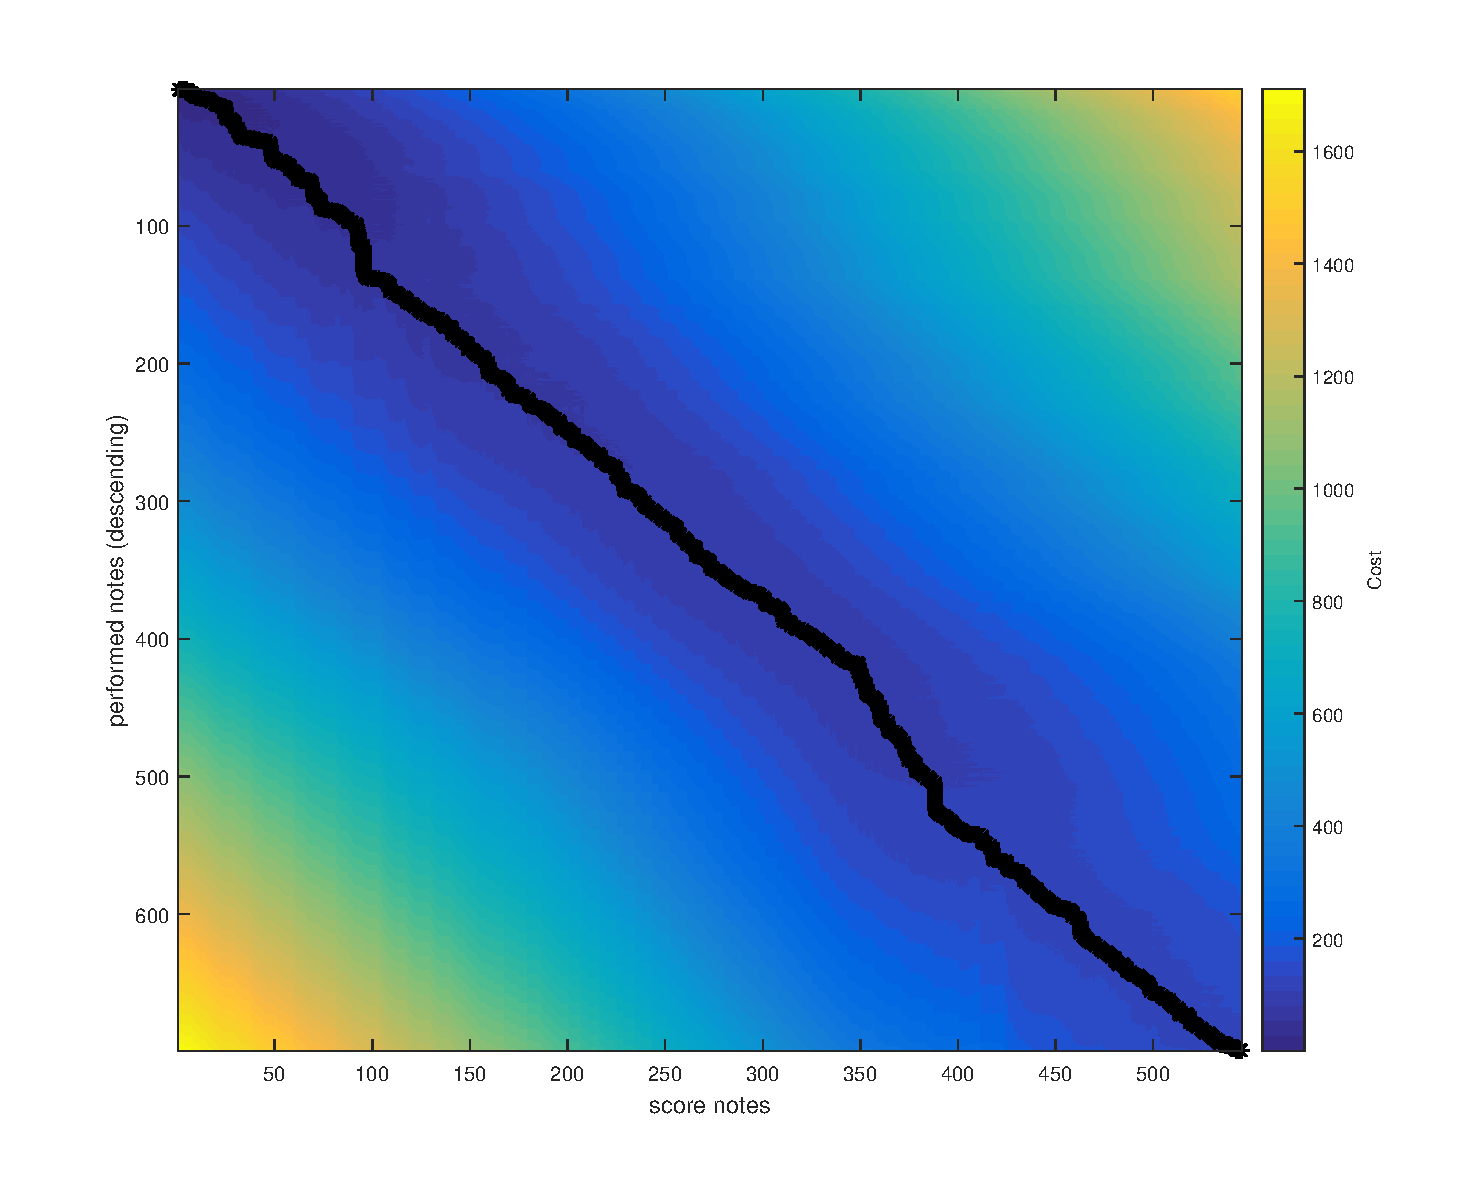
\includegraphics[width=0.8\textwidth]{Figures/Suite_en_la_cost.pdf}
\end{figure}

Some restrictions have been done to this optimal path computation in order to apply some rules. Horizontal paths are forbidden in order to ensure that each performance note has only one score note as reference, and be able to compute embellishments. However, we need to allow vertical paths so one score note can be played as several performance notes. In figure~\ref{fig:darn_auto_alignment} we can see an example of an automatic performance to score alignment. In this plot, score has been shifted two octaves up in order to have a better visualization.

\begin{figure}[ht!]
\caption{\textit{Darn that dream} performance to score alignment}
\label{fig:darn_auto_alignment}
\centering
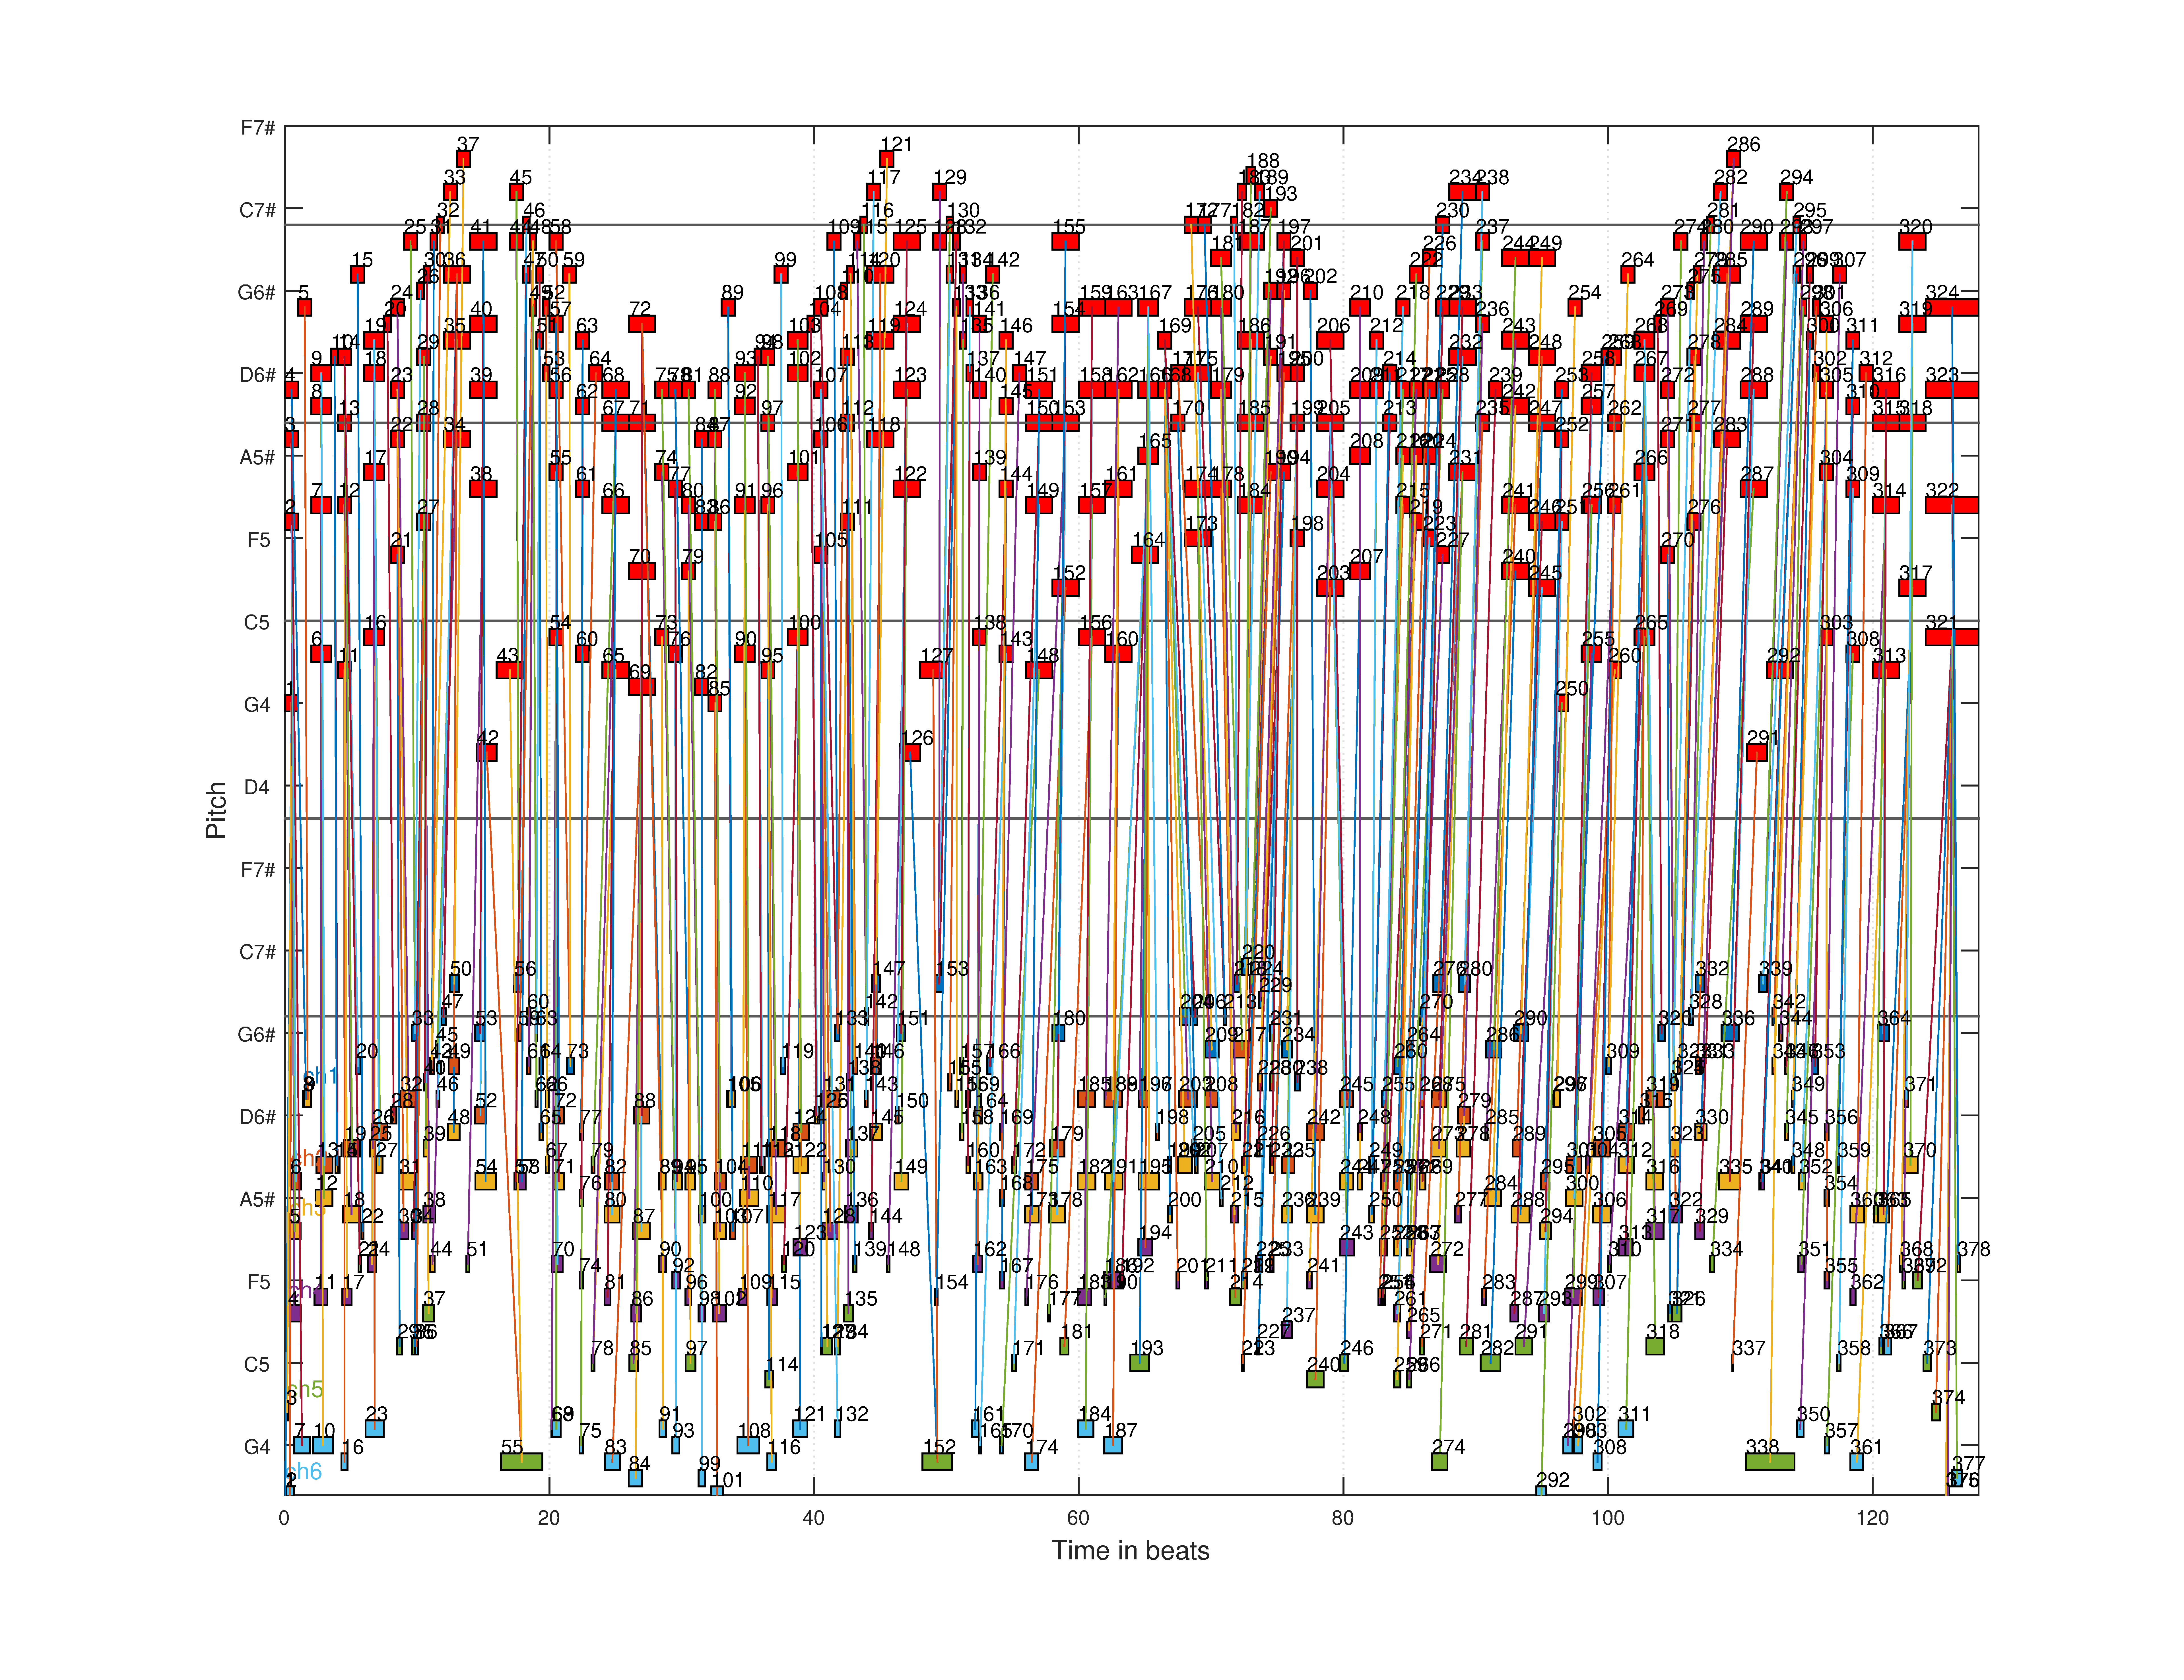
\includegraphics[width=\textwidth]{Figures/Darn_that_dream_auto.pdf}
\end{figure}


\subsection{Performance actions}

\section{Machine Learning modelling}
\cleardoublepage

